% This must be in the first 5 lines to tell arXiv to use pdfLaTeX, which is strongly recommended.
\pdfoutput=1

\documentclass[11pt]{article}

% Remove the "review" option to generate the final version.
\usepackage[]{ACL2023}

\usepackage{fancyhdr} % For customizing headers and footers
\pagestyle{fancy}
\fancyhf{} % Clear all header and footer fields
\fancyfoot[C]{\thepage} % Add page number in the center of the footer
\usepackage{times}
\usepackage{latexsym}
\usepackage[T1]{fontenc}
\usepackage[utf8]{inputenc}
\usepackage{microtype}
\usepackage{inconsolata}
\usepackage{hyperref}
\usepackage{amsmath}
\usepackage{graphicx}
\usepackage[table,xcdraw]{xcolor}
\usepackage{float}
\setlength\titlebox{5cm}

\title{Comparative Analysis of BERT,\\sciBERT and secBERT Fine-Tuning\\for Cybersecurity Technique Classification}

\author{Michael Garrett \\
  w266 - Natural Language Processing \\
  Masters of Information and Data Science \\
  University of California, Berkeley \\
  \texttt{\href{mailto:m.garrett@ischool.berkeley.edu}{m.garrett@ischool.berkeley.edu}}}

\date{\today}

\begin{document}
\maketitle
\begin{abstract}
The increasing sophistication of cybersecurity attacks underscores the need for advanced methods to detect and categorize threat techniques effectively. This experiment evaluates the performance of three pretrained transformer models—BERT, sciBERT, and secBERT—fine-tuned for classifying cybersecurity techniques according to the MITRE Threat Report Attack Mapping (TRAM) framework. Contrary to expectations, BERT performed comparably to secBERT, even though secBERT is specialized for security texts. Both models achieved F1 scores ranging between 0.89 and 0.90. A tight diagonal in the confusion matrices indicates balanced precision and recall, suggesting a well-calibrated model performance. However, potential issues such as model saturation, differences in tokenization, and data quality may have influenced these results. This study highlights the effectiveness of BERT and sciBERT in handling cybersecurity classification tasks and emphasizes the need for further exploration into model training and data augmentation strategies to improve threat classification accuracy.
\end{abstract}


\section{Introduction}

The increasing frequency and sophistication of cybersecurity attacks necessitate advanced methods for detecting and categorizing cybersecurity techniques used by threat actors. One such method is the classification of Cyber Threat Intelligence (CTI) reports to the MITRE ATT\&CK Framework (MAF) techniques. MAF is a comprehensive knowledge base of adversarial tactics and techniques used in cybersecurity, designed to help CTI analysts interpret cyber threats and adversarial behavior \cite{hubbard2020measuring}. The MITRE Corporation understood this need and created the Threat Report Attack Mapping (TRAM) framework \cite{tram}. TRAM is a tool designed to map threat reports to MAF techniques. It represents a significant advancement in automating the analysis of cybersecurity threat reports. By systematizing the mapping of threat reports to the MAF, TRAM enhances the accuracy and efficiency of threat intelligence processes. This automation reduces the manual effort required from analysts, allowing them to focus on more complex tasks. Leveraging state-of-the-art NLP models to enhance the TRAM framework's efficacy in classifying and understanding cybersecurity techniques could provide substantial benefits to the cybersecurity community.

In this study, I conducted a comparative analysis of three pretrained transformer models—BERT, sciBERT, and secBERT—each fine-tuned specifically for classifying cybersecurity techniques according to the MITRE TRAM framework. BERT, the Bidirectional Encoder Representations from Transformers, has set a new standard for NLP tasks due to its deep bidirectional understanding of context. The sciBERT, a BERT variant pretrained on scientific text, model is tailored for tasks requiring domain-specific knowledge found in scientific literature. The secBERT, another BERT variant, model is specialized for security-related texts, making it potentially more effective for cybersecurity applications.

My research aims to evaluate the performance of these models in the context of classifying cybersecurity techniques. I seek to answer the following key questions:

\begin{itemize}
	\item How does the baseline performance of BERT, SciBERT, and SecBERT compare on a cybersecurity technique classification task?
	\item What improvements in classification performance can be achieved through fine-tuning a model that is pretrained on cybersecurity corpora?
\end{itemize}

By building and comparing these models, I strive to identify the most effective approach for enhancing the MITRE TRAM framework's capability to automatically classify and understand cybersecurity techniques. This work contributes to the broader effort of improving cybersecurity threat analysis through advanced NLP techniques and provides valuable insights into the strengths and limitations of different transformer-based models in a specialized domain. Additionally, the findings could guide future developments in automated threat intelligence systems, ensuring they are more accurate and responsive to emerging threats. Ultimately, this research seeks to enhance the overall efficacy of cybersecurity defenses by providing more precise and timely threat classifications.

\section{Background}

In December 2019, MITRE introduced the inaugural version of the Threat Report Attack Mapping (TRAM) Framework, referred to as TRAM V1. This initial iteration employed a logistic regression model to classify cybersecurity threat reports, using word frequencies and the full set of MITRE ATT\&CK techniques as input features for the classifier. 

In a significant advancement four years later, MITRE released TRAM Version 2 (V2), which marked a notable enhancement over its predecessor. TRAM V2 incorporated a transformer-based architecture, specifically sciBERT, to leverage the model's ability to capture complex contextual relationships in text. This upgrade improved the model's performance by employing a more sophisticated approach to feature extraction and classification. Additionally, TRAM V2 focused on a curated subset of fifty techniques from the ATT\&CK knowledge base, optimizing the classifier’s accuracy and relevance. This evolution reflects a broader trend in cybersecurity threat analysis towards adopting advanced NLP techniques to better handle the nuances and complexities of threat data, thereby improving the framework’s overall effectiveness in mapping and interpreting adversarial tactics.

The idea of improving model performance through domain-specific pretraining was explored in a significant paper titled "SciBERT: A Pretrained Language Model for Scientific Text" by \cite{beltagy2019scibert}, published in 2019. This paper demonstrated how pretraining BERT on scientific literature improved performance on scientific text classification and other related tasks. This concept has since been expanded to various domains, showing that domain-specific pretraining can enhance performance in specialized text classification tasks. This motivated the creation of secBERT. 

SecBERT is a specialized variant of BERT tailored specifically for cybersecurity applications. It is fine-tuned on a domain-specific corpus that includes a diverse range of security-related texts, such as threat reports, vulnerabilities, and attack patterns. By leveraging BERT’s deep bidirectional transformer architecture, secBERT is designed to capture and understand the intricate details and contextual nuances within cybersecurity-related language. This fine-tuning process enhances secBERT’s ability to accurately interpret and classify cybersecurity threats, making it a valuable tool for automating the analysis of security data and improving the detection and categorization of adversarial techniques. The model’s domain-specific training allows it to perform more effectively in cybersecurity contexts compared to general-purpose language models, offering improved performance in tasks such as threat intelligence and vulnerability assessment.

I plan to use secBERT for fine-tuning similarly to how TRAM applied sciBERT. The literature suggests that this approach should improve the accuracy of predicting MAF techniques from a given sentence. This study aims to build on this foundation by offering a thorough comparative analysis of these models specifically for the classification of cybersecurity techniques.

Notable works in the field include:

\begin{itemize}
	\item \textbf{BERT}: Developed by \cite{devlin2018bert}Devlin et al., BERT has been a breakthrough in NLP due to its bidirectional transformer architecture. It has achieved state-of-the-art results in many tasks including text classification.
	\item \textbf{SciBERT}: Introduced by \cite{beltagy2019scibert}, SciBERT is pretrained on a large corpus of scientific text, making it more adept at handling domain-specific terminology.
        \item \textbf{SecBERT}: Created by \cite{secBERT}, although less documented in academic literature, SecBERT is a specialized variant fine-tuned on cybersecurity texts, aiming to capture the nuances of this domain.
\end{itemize}

\section{Methods}

To determine if a pretrained model such as secBERT can outperform the baseline BERT and sciBERT models in the task of text classification on cybersecurity data, I needed to ensure as many variables were consistent as possible to establish a fair comparison. My approach was to use the design that MITRE applied to fine-tune their sciBERT model and apply it to all three of my models. This included attempting to get the data into the same shape as the data used in training their model, building the model architecture as close as possible to theirs, and using the same evaluation metrics that they reported. 

\subsection{Data}

The dataset I acquired appears to have been curated using the MAF techniques available around the early part of 2022. I found it on HuggingFace, and it consists of 14.4k human-labeled rows. Unfortunately, the data card details were not filled out by the owner \cite{data} so there are no details on how the data was collected. 

The ATT\&CK knowledge base regularly expands as adversaries continuously develop and employ new techniques. New techniques are often initially documented by only a small number of CTI reports. MAF adds a new technique based on just one public report of a new behavior. However, the limited reporting on these new techniques can lead to inaccurate results and an extremely unbalanced dataset.

This is a well understood problem in the industry as \cite{grigorescu2022cve2att} discovered in their paper titled "CVE2ATT\&CK: BERT-Based Mapping of CVEs to MITRE ATT\&CK Techniques." Their aim was to develop a model that leverages the textual description found in CVE (Common Vulnerabilities and Exposures) metadata to create strong correlations with the MITRE ATT\&CK techniques. They utilized two approaches which I implemented in the handling of my data. 

The first approach was removing the techniques with the lowest frequency. Based on my dateset, I removed the lowest frequencies of less than 100. By doing so I went from 190 techniques to 44. Although this may seem drastic, its important to note that TRAM V2 uses only 50 of the most common techniques in the training of sciBERT. 

The second approach was to upsample the remaining lower frequency techniques. Grigorescu, et. al. used a framework called TextAttack for data augmentation. The TextAttack Framework is an open-source library designed for generating and evaluating adversarial attacks on natural language processing (NLP) models. The data augmentation feature can systematically generate variations of texts that belong to low-frequency classes. An example is provided in Appendix \ref{sec:data}. This can help to balance the dataset and provide more training and test examples for these underrepresented classes. I chose a threshold of 200 so that at most a single class would be composed of 50\% of augmented data. Additionally, I downsampled the highest frequency techniques to 500. Only two techniques were impacted by the downsampling (T1059 and T1027). This resulted in an increase in dataset from the original 14.4k to 15.2k rows. This is still significantly lower than the 26.6k rows MITRE acquired for the TRAM V2 project. See Appendix \ref{sec:prep} for histograms of data preprocessing. 

The dataset was split into three parts: 80\% for training, 10\% for validation, and 10\% for testing. This ensured that the models were trained on a large portion of the data while still allowing for thorough evaluation and validation of their performance. This split is consistent with the approach MITRE took for TRAM V2. The splits were shuffled and saved off as CSVs to my Google Drive so that each of the models would use the exact same data. 

\subsection{Models}

All models were created by standardizing on the hyperparameters used in the TRAM V2 finetuning of sciBERT. See Table \ref{tab:hyperparameters} for a list of the hyperparameter and its corresponding values. I attempted to limit the deviations between the models but, as it is explained below, this was not always possible. 

\begin{table}[h]
\centering
\begin{tabular}{lc}
\hline
\rowcolor[HTML]{C0C0C0} 
\textbf{Hyperparameters} & \textbf{Values} \\ \hline
max\_length & 512 \\
batch\_size & 10 \\
epcochs & 5 \\
learning\_rate & 2e-5 \\ \hline
\end{tabular}

\caption{Standardized Hyperparameter Values used on all three models.}
\label{tab:hyperparameters}
\end{table}

Additionally, the computational resources used for all three models included a T4 GPU offered via Google Colab's runtime environment. The option to utilize high-RAM was necessary as the first run of BERT on the data failed due to running out of memory.

\subsubsection{Baseline - BERT}
The baseline model is the BERT model. Using the pretrained 'bert-base-cased' from HuggingFace, I was able to build a model using TensorFlow. I initially planned to build a single notebook for all three models, but technical issues forced me to use PyTorch for the sciBERT and secBERT models.

To stay consistent with the TRAM V2 project I used the TFBertForSequenceClassification transformer. This is the TensorFlow equivalent of the BertForSecqunceClassification tranformer used by MITRE. This HuggingFace transformer includes a classification head (softmax) on top of a pooled output layer. Having these layers in a single pretrained transformer simplified the creation of all three models. 

Another notable difference to the baseline is the use of Adam as the optimizer. The choice to use Adam for the optimizer, instead of AdamW, was a technical one. AdamW is an extension of Adam that includes decoupled weight decay regularization. This helps prevent overfitting by adding a penalty to the loss function proportional to the sum of the squared weights. See \cite{loshchilov2017decoupled} for a thorough explanation.

I chose to keep the Adam weight decay (L2 regularization) at the default value of 0 because matching it to the AdamW optimizer would affect the gradients during backpropagation. Since AdamW decouples weight decay from gradiant updates, I felt this was the best approach to ensure somewhat of a level playing field. The default value for the epsilon parameter was used in both sciBERT and secBERT.  

\subsubsection{TRAM - sciBERT}

Since TRAM used the sciBERT model as their classifier, I built and trained my own sciBERT model fine-tuned on my dataset. I wanted to see if I could get close to the results they published. This could gauge whether I was mimicking their experiment. I used the same model they used, 'allenai/scibert\_scivocab\_uncased', and the BERTForClassification transformer. Like the TRAM project, I used the PyTorch library to build out this model. I deviated from their codebase and wrote my own code that made sense to me, however, none of those changes should have impacted the outcome. 

\subsubsection{Experiment - secBERT}

Once I built out the notebook for sciBERT, building the secBERT model was as simple as changing the model name to 'jackaduma/SecBERT'. Everything else, even the code, remained the same. 

Evaluateing the architecture of the models I noticed that secBERT was different than sciBERT in the following ways:

\begin{itemize}
	\item \textbf{Embeddings}: The sciBERT model has a vocabulary size of 31,090 tokens, while secBERT has a larger vocabulary size of 52,000 tokens. The secBERT model supports slightly longer sequences with 514 position embeddings compared to 512 in sciBERT. The sciBERT model uses 2 token types (typically for distinguishing between segments in sentence-pair tasks), whereas secBERT uses only 1 token type.
	\item \textbf{Encoder}: The scitBERT model has a deeper encoder with 12 layers compared to secBERT's 6 layers.
        \item \textbf{Attention}: Both models use similar attention mechanisms, but the depth of the encoder (number of layers) leads to a significant difference in their representational capacities.
\end{itemize}

These differences imply that sciBERT is designed to handle more complex tasks with a deeper architecture and larger vocabulary, whereas secBERT is optimized for tasks requiring shorter sequences and a simpler model. These implicit differences within the models themselves may manifest in the results. 

\subsection{Metrics}

Evaluation metrics such as precision, recall, and F1-score were employed to assess the performance of each model. This is in-line with those reported by MITRE. I choose to add accuracy for additional comparison and F2-score to the evaluation metrics. 

\begin{equation}
    F_{\beta} = (1 + \beta^2) \cdot \frac{\text{precision} \cdot \text{recall}}{(\beta^2 \cdot \text{precision}) + \text{recall}}
\end{equation}

The F2-score gives more weight to recall than precision. This is valuable when the cost of missing positive instances (false negatives) is higher than the cost of false positives. For instance, in medical diagnosis, missing a disease might be more critical than falsely identifying it. The same applies to the classification of cybersecurity techniques. Missing the classification of a technique results in inaction, whereas falsely classifying a technique. Although not ideal, this results in verifying detection of such a technique.  

Based on the literature, secBERT is likely to be the optimal model for classifying CTI text to MAF techniques compared to BERT and sciBERT, due to its training on a cybersecurity-related text corpus. My hypothesis is that, by standardizing the model architecture and data, I can show that secBERT will outperform the other models. If this hypothesis is confirmed, it would be essential to fine-tune production models on secBERT to enhance the performance of tools used by cybersecurity analysts. 

\section{Results \& Discussion}

After fine-tuning all three models the results were quite unexpected, as shown in Table \ref{tab:results}. I anticipated a superior performance of sciBERT and secBERT over the baseline BERT model in the task of cybersecurity technique classification. However, BERT performed equally as well as secBERT achieving the same F1 score. In fact, the range of the metrics is 0.89-0.90 for all models. Although secBERT outperformed the other two models in all metrics the race was quite tight. 

\begin{table}[h]
\centering
\resizebox{\columnwidth}{!}{%
\begin{tabular}{l|c|c|c|c|c}
\hline
\rowcolor[HTML]{C0C0C0} 
\textbf{Model} & \textbf{\begin{tabular}[c]{@{}c@{}}Test\\ Acc\end{tabular}} & \textbf{Precision} & \textbf{Recall} & \textbf{F1} & \textbf{F2} \\ \hline
Baseline - BERT & 0.90 & 0.90 & 0.90 & \textbf{0.90} & 0.89 \\
TRAM - secBERT & \textbf{0.91} & \textbf{0.91} & \textbf{0.91} & \textbf{0.90} & \textbf{0.90} \\
Experiment - sciBERT & 0.90 & 0.89 & 0.89 & 0.89 & 0.89
\end{tabular}%
}
\caption{Results from 3 models.}
\label{tab:results}
\end{table}

In terms of precision and recall, both metrics were equal and consistently high across all three models. This equality indicates that the models have balanced performance regarding false positives and false negatives, which is beneficial in scenarios where both types of errors carry similar costs. Because precision equals recall, the F1 score—defined as the harmonic mean of precision and recall—will also equal the value of precision (or recall).

I aimed to identify the F2 score, which prioritizes recall over precision, to measure scenarios where missing relevant instances is more critical than including irrelevant ones. However, since precision and recall are equal for all three models, the F2 score calculation results in the same value as the F1 score.

\begin{enumerate}
    \item F1 score when P = R:
    \begin{equation}
    F1 = 2 \cdot \frac{P \cdot P}{P + P} = 2 \cdot \frac{P^2}{2P} = 2 \cdot \frac{P}{2} = P
    \end{equation}

    \item F2 score when P = R:
    \begin{equation}
    F2 = 5 \cdot \frac{P \cdot P}{4P + P} = 5 \cdot \frac{P^2}{5P} = 5 \cdot \frac{P}{5} = P
    \end{equation}
\end{enumerate}

Ultimately, I believe my experiment is flawed for two main reasons. First, I used a pretrained model from HuggingFace that was claimed to have been trained on a relevant cybersecurity corpus. However, I have no way to verify whether this claim is accurate or if the training was done properly. If I had the resources and time, I would consider training a model myself to ensure its claims are valid. 

On the other hand, the model might already be highly optimized for the domain on which it was trained, meaning that further optimization may not yield significant improvements. This concept of model saturation could explain why the training curves appeared flat. It might also clarify why the predictions on the training set were reasonably good. The confusion matrix in Appendix \ref{sec:cm} shows a tight diagonal, indicating high accuracy and supporting this explanation. If this is the case, it is interesting that by fine-tuning BERT or sciBERT you can achieve similar or a slightly better performance. 

The second reason this experiment is flawed is that SecBERT differs significantly from BERT and SciBERT. This difference is evident not only in the aspects I discussed in the models section 3.2 \textit{supra} (such as embeddings, encoder, and attention mechanisms), but also in its text tokenization approach. As shown in Appendix \ref{sec:fillmask}, the tokenization process varies: there is no CLS token at the beginning or SEP token at the end of the text. Instead, a <s> token is used in both positions. Given the importance of the CLS token for classification tasks, I am interested in how these differences, along with other design choices made by the creator, might affect the results.

One possibility is that the data I used was of poor quality. Using the TextAttack to augment some of the existing data could have trained the models overfit. Although I do not believe this to be the case. As \cite{grigorescu2022cve2att} demonstrated in the results section of their report, the F1 score increased when data augmentation was used on all three models. 

An error analysis was conducted to further understand the misclassifications made by each model. The analysis revealed that domain-specific terminology and context, which are prevalent in cybersecurity texts, were better handled by BERT and sciBERT. These models were more adept at interpreting and categorizing complex and technical language, highlighting their suitability for specialized NLP tasks. Observing the confusion matrices in Appendix \ref{sec:cm}, one can simply observe that the squares in the diagonal are a lighter color indicating less accuracy. 

\section{Conclusion}

In conclusion, the comparative analysis of BERT, sciBERT, and secBERT for cybersecurity technique classification revealed that BERT performed as well as secBERT, despite expectations that the latter would excel due to its specialization. The close performance across all models, with F1 scores ranging from 0.89 to 0.90, suggests that the models achieved balanced precision and recall, but did not exhibit significant differences in classification efficacy. The experiment's results highlight potential issues with model saturation and differences in tokenization strategies, particularly with secBERT, which may have impacted performance. Additionally, the quality of the data used for fine-tuning could have influenced the outcomes, though data augmentation showed promise in similar studies. Overall, while the findings provide insight into the effectiveness of these models, they also underscore the need for further investigation into model training and data quality to enhance the classification of cybersecurity techniques.


% Entries for the entire Anthology, followed by custom entries
\bibliography{custom}
\bibliographystyle{acl_natbib}

\appendix
\section{Data Augmentation}
\label{sec:data}

The table on the following page illustrates an example of how a row of data was augmented using TextAttack. This augmentation process involves generating variations of the original text to enhance the model's robustness and performance. The table shows the original row alongside its augmented versions, demonstrating the types of modifications made to create more diverse training examples. These modifications help improve the model's ability to generalize by exposing it to a broader range of text inputs during training.

\begin{table*}[h]
\centering
\begin{tabular}{|l|l|}
\hline
\rowcolor[HTML]{C0C0C0} 
\multicolumn{1}{|c|}{\cellcolor[HTML]{C0C0C0}\textbf{Technique}} & \multicolumn{1}{c|}{\cellcolor[HTML]{C0C0C0}\textbf{Text}} \\ \hline
Original & Chimera has used net user for account discovery. \\ \hline
Replacement & Chimera has used net user for score discovery. \\ \hline
Removal & has used net user for account discovery. \\ \hline
Insertion & Chimera has profits used net user for account discovery. \\ \hline
Swap & Chimera has used discovery user for account net. \\ \hline
\end{tabular}
\caption{Example of TextAttack's data augmentation techniques.}
\label{tab:data-augmentation}
\end{table*}

\clearpage
\section{Data Preprocessing}
\label{sec:prep}

\begin{enumerate}
    \item \textbf{Original Dataset Distribution} (Figure \ref{fig:og}):
    
    The first histogram depicts the distribution of classes in the original dataset. Each bar represents the number of instances for each class, illustrating the initial imbalance with varying class frequencies. Some classes have high frequencies, while others are sparsely represented, providing a baseline for understanding the dataset's initial state.
    \item \textbf{Post-Trimming Distribution} (Figure \ref{fig:trimmed}):
    
    The second histogram shows the class distribution after trimming. In this stage, classes with fewer than 100 instances have been removed. The histogram reveals a more focused dataset with reduced class diversity, highlighting the effect of excluding underrepresented classes. This step aims to eliminate noise and improve model training efficiency by concentrating on more substantial classes.
    \item \textbf{Post-Upscaling Distribution} (Figure \ref{fig:upscaled}):
    
    The third histogram illustrates the class distribution after applying data augmentation techniques using TextAttack. Here, classes with fewer than 200 instances have been upscaled to increase their representation in the dataset. The histogram reflects the growth in frequency for these previously underrepresented classes, demonstrating the impact of augmentation in balancing the dataset and providing a more uniform distribution of classes.
    \item \textbf{Final Distribution} (Figure \ref{fig:final}):
    
    The fourth histogram presents the final distribution after downscaling the two largest classes to a maximum of 500 instances each. This final adjustment ensures that no class dominates the dataset, leading to a more balanced representation. The histogram shows a dataset with equalized class frequencies, facilitating a fair evaluation of the model's performance across all classes and reducing the risk of bias towards overrepresented classes.
\end{enumerate}

These histograms collectively illustrate the transformation of the dataset from its initial state through various preprocessing steps, including trimming, upscaling, and downscaling, culminating in a balanced distribution suitable for model training and evaluation.

\begin{figure*}[h]
    \centering
    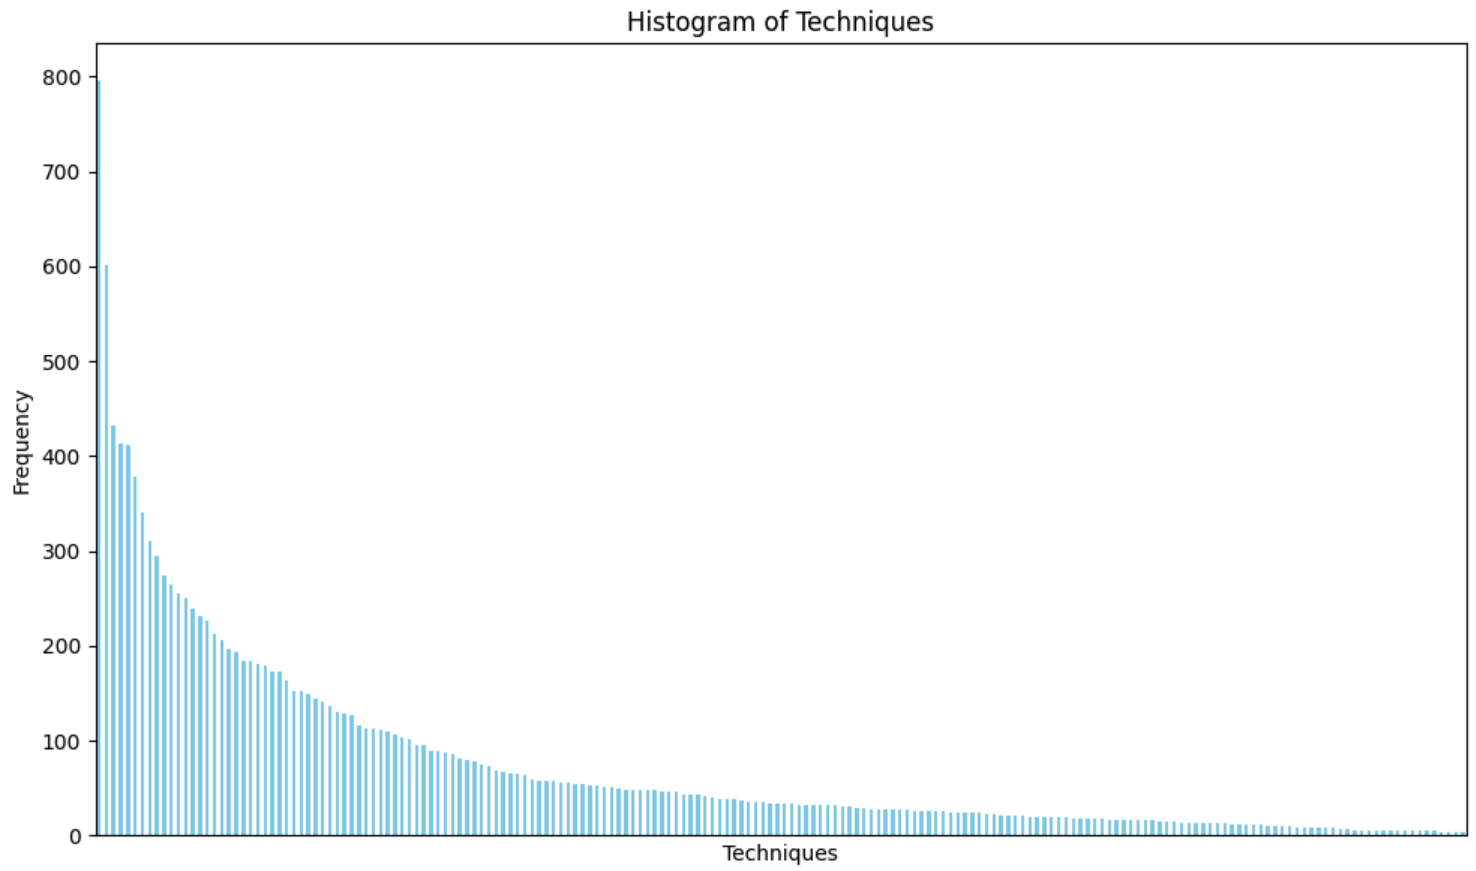
\includegraphics[width=1\linewidth]{original.png}
    \caption{Original Distribution of the data before any preprocessing.}
    \label{fig:og}
\end{figure*}

\begin{figure*}[h]
    \centering
    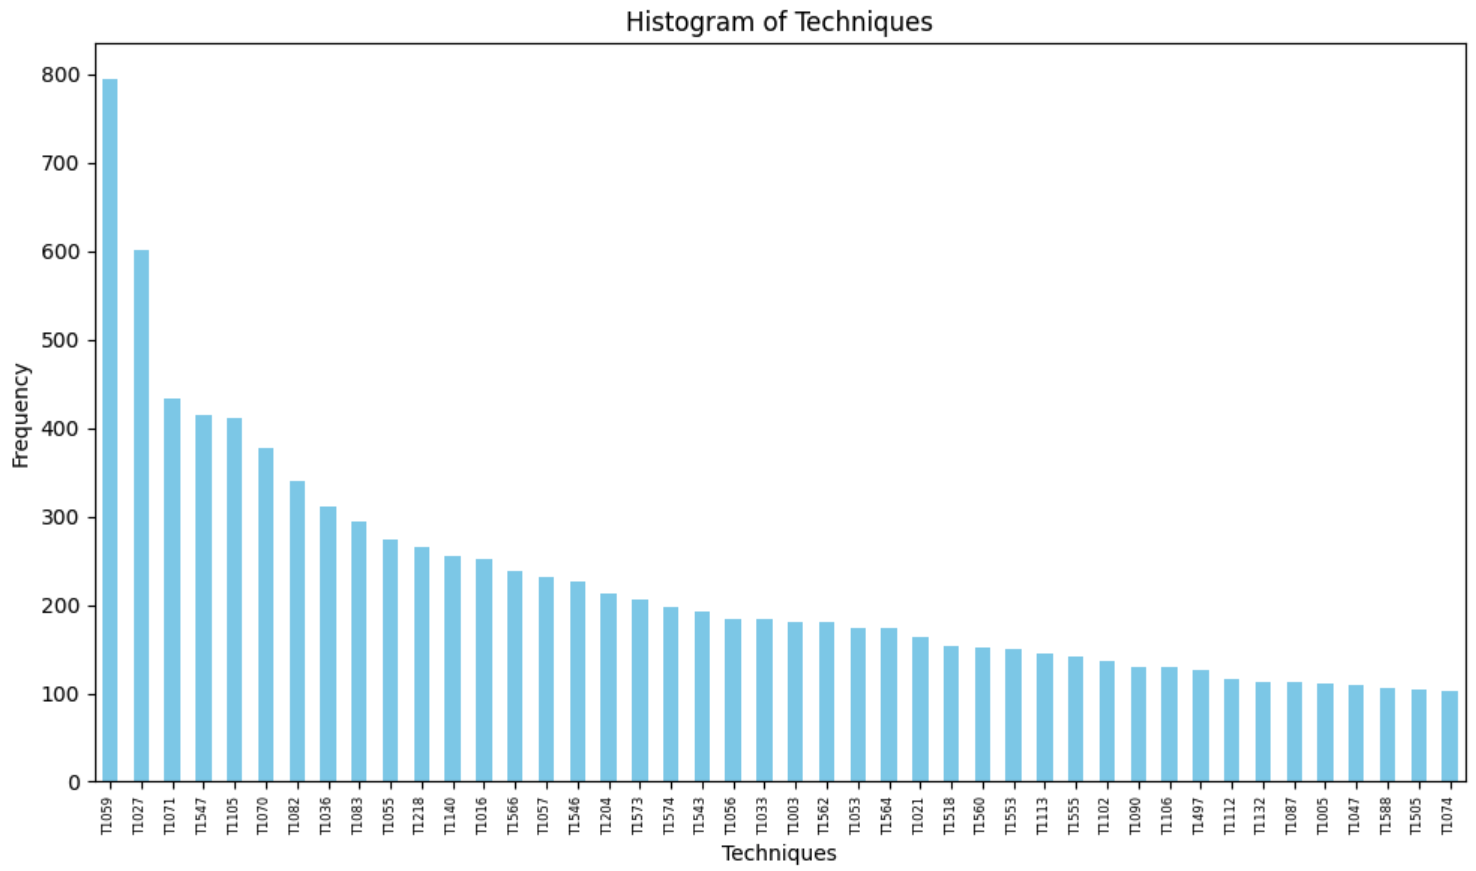
\includegraphics[width=1\linewidth]{trimmed.png}
    \caption{Distribution after removing the techniques with less than 100 counts.}
    \label{fig:trimmed}
\end{figure*}
\clearpage
\begin{figure*}[h]
    \centering
    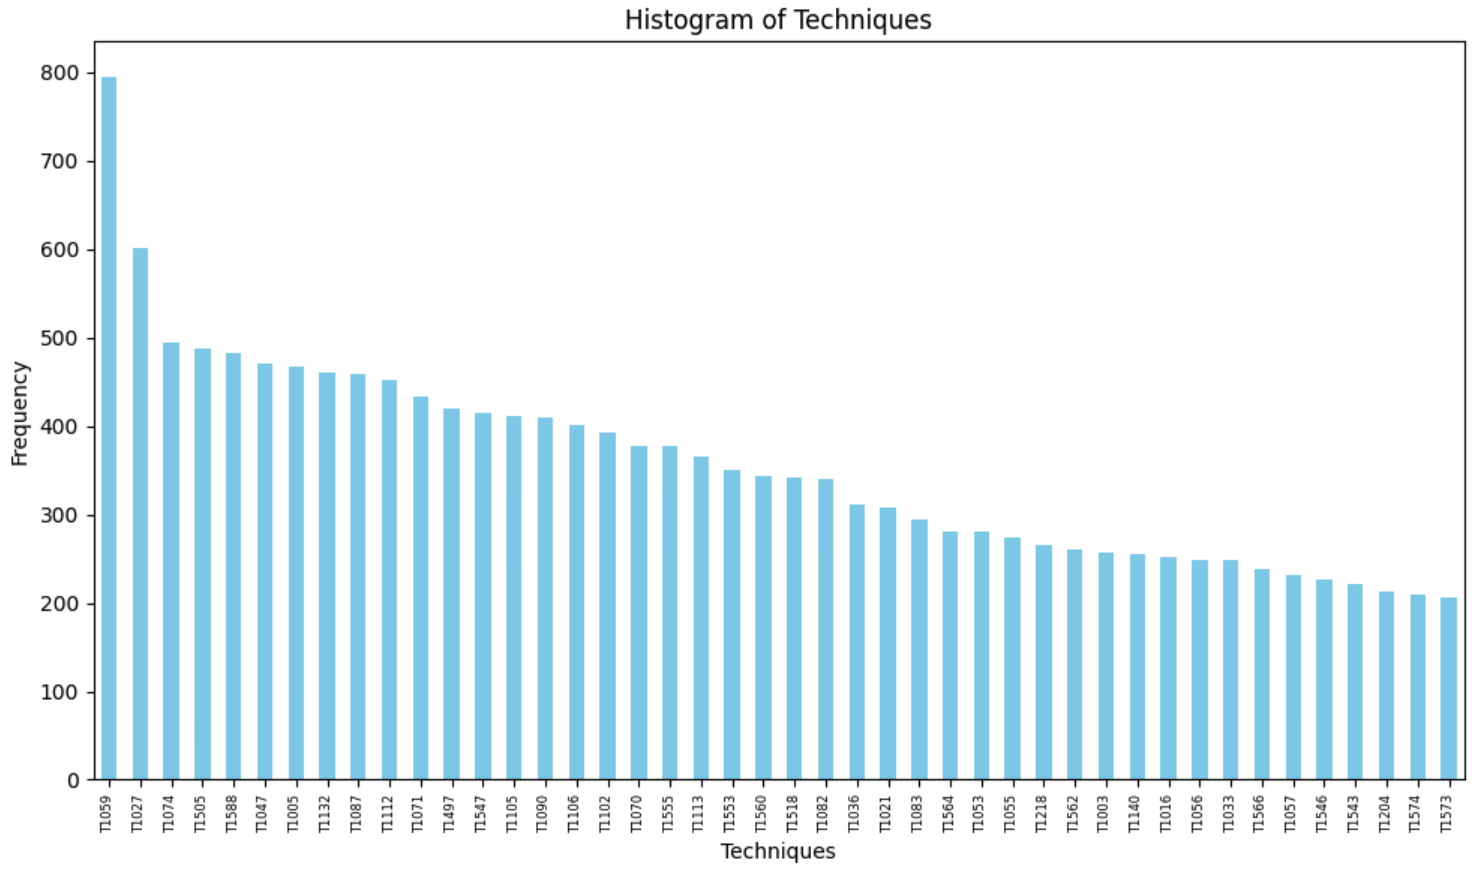
\includegraphics[width=1\linewidth]{upsampled.png}
    \caption{Distribution after upsampling using data augmentation techniques.}
    \label{fig:upscaled}
\end{figure*}

\begin{figure*}[h]
    \centering
    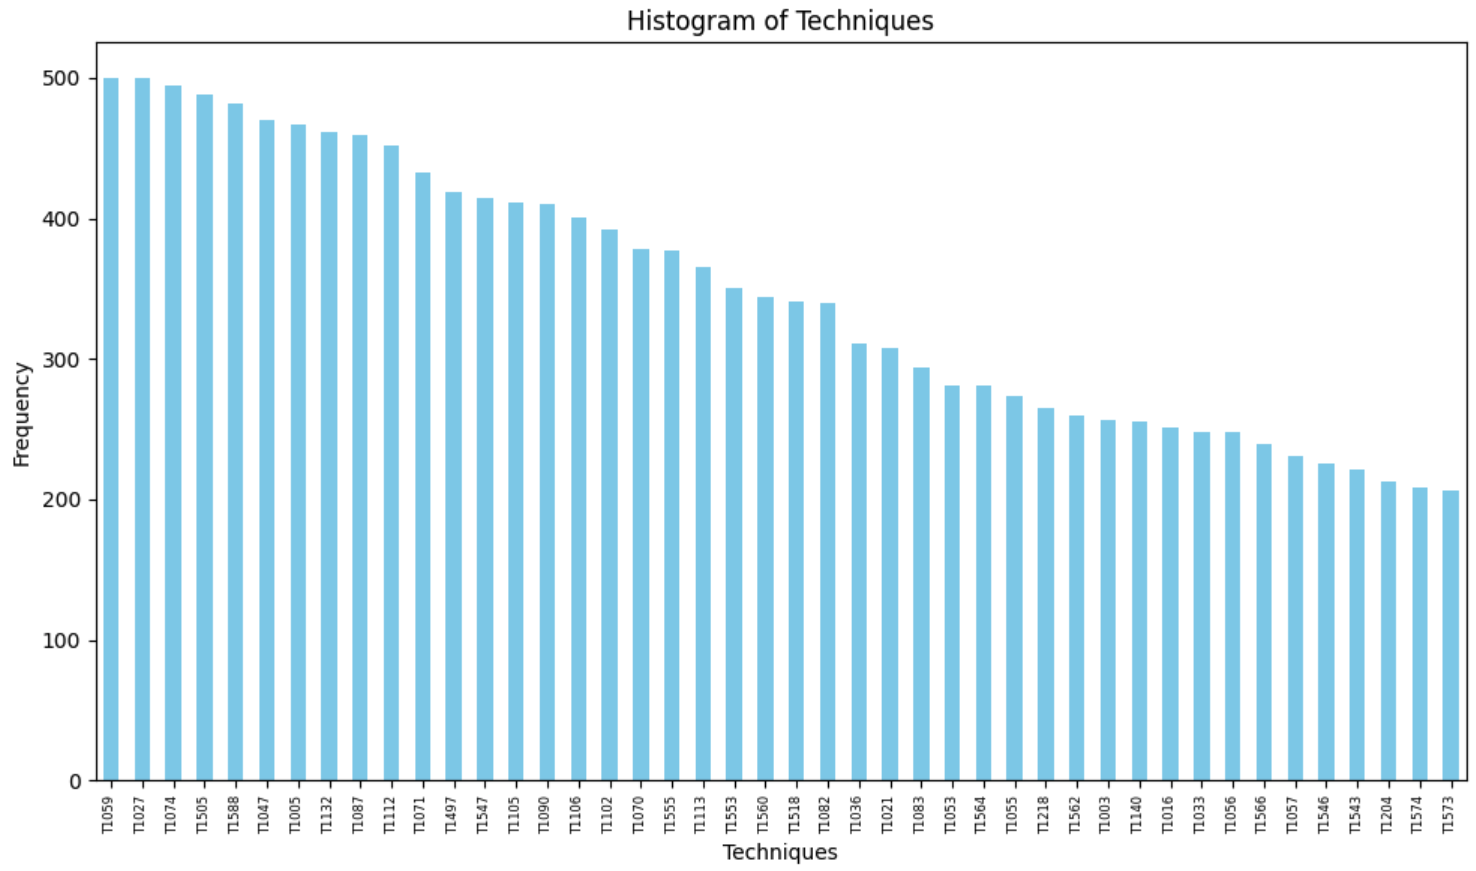
\includegraphics[width=1\linewidth]{final.png}
    \caption{Final distribution of data.}
    \label{fig:final}
\end{figure*}

\clearpage
\section{Fill Mask Differences}
\label{sec:fillmask}
\begin{figure}[h]
    \centering
    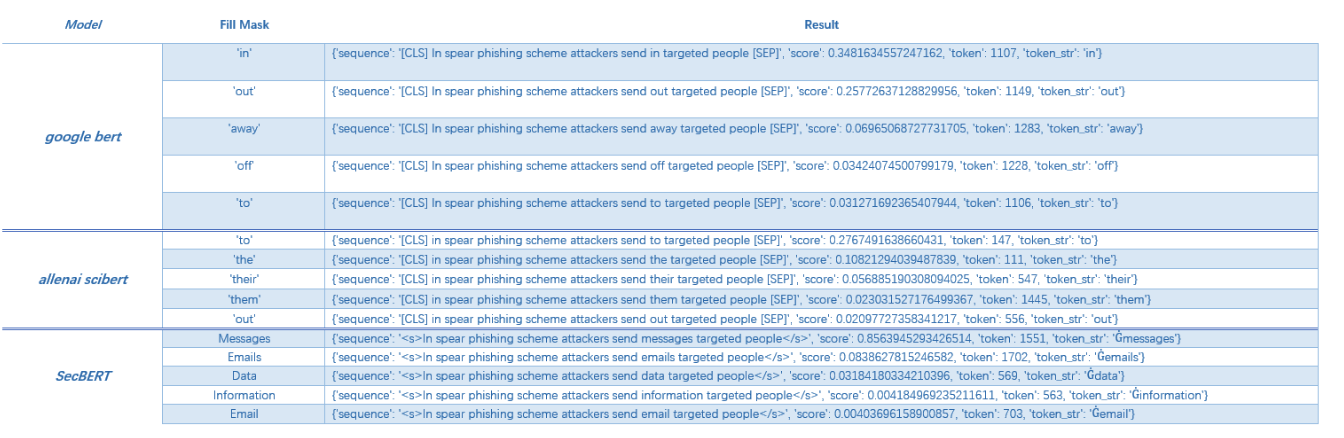
\includegraphics[width=2.2\linewidth]{fill-mask.png}
    \caption{Fill-Mask differences between models.}
    \label{fig:fill-mask}
\end{figure}

\clearpage
\section{Confusion Matrices}
\label{sec:cm}

\begin{enumerate}
    \item Confusion Matrix 1 \ref{fig:cm-baseline}:

    The first confusion matrix displays a tight diagonal, indicating that the model's predictions closely align with the actual class labels across most categories. The diagonal squares are uniformly colored, showing consistent accuracy in classifying each class correctly. This matrix reflects a model with high performance, with the majority of predictions being correct and only minimal misclassifications.
    \item Confusion Matrix 2 \ref{fig:cm-scibert}:

    The second confusion matrix also exhibits a tight diagonal, similar to the first matrix. The diagonal squares are similarly colored, indicating comparable accuracy levels. This matrix demonstrates that the model performs consistently well across various classes, maintaining a high level of correctness in predictions. The uniform coloring of the diagonal reinforces the model's reliable performance and balanced accuracy.
    \item Confusion Matrix 3 \ref{fig:cm-secbert}:

    The third confusion matrix shows a tight diagonal as well but with noticeable lighter patches within the diagonal squares. These lighter areas indicate reduced accuracy in some classes compared to the first two matrices. While the overall diagonal remains tight, the presence of lighter patches suggests that the model struggles more with certain classes, resulting in lower accuracy for those specific categories. This matrix highlights areas where the model's performance could be improved, pointing to potential weaknesses in classification for specific classes.
\end{enumerate}

Together, these confusion matrices illustrate the model's accuracy across different classes, with the first two matrices showing high and consistent performance, while the third matrix reveals areas of reduced accuracy, indicating the need for further analysis to address the performance gaps.

\begin{figure*}[h]
    \centering
    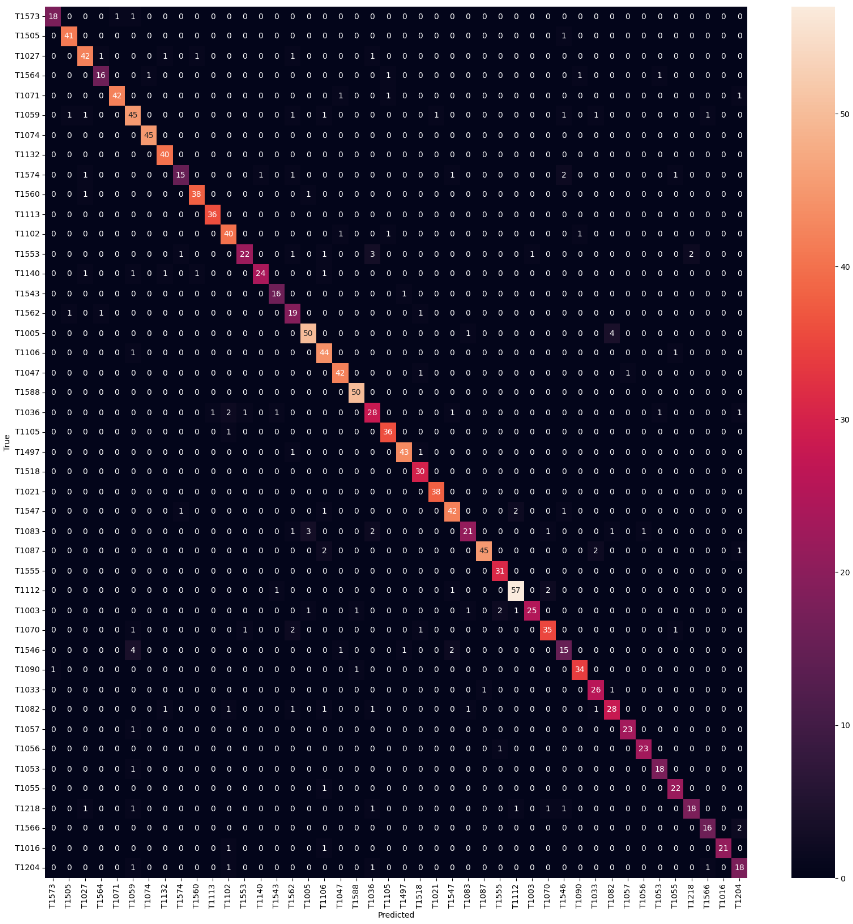
\includegraphics[width=1\linewidth]{baseline_confution_matrix.png}
    \caption{BERT Confusion Matrix}
    \label{fig:cm-baseline}
\end{figure*}
\clearpage
\begin{figure*}[h]
    \centering
    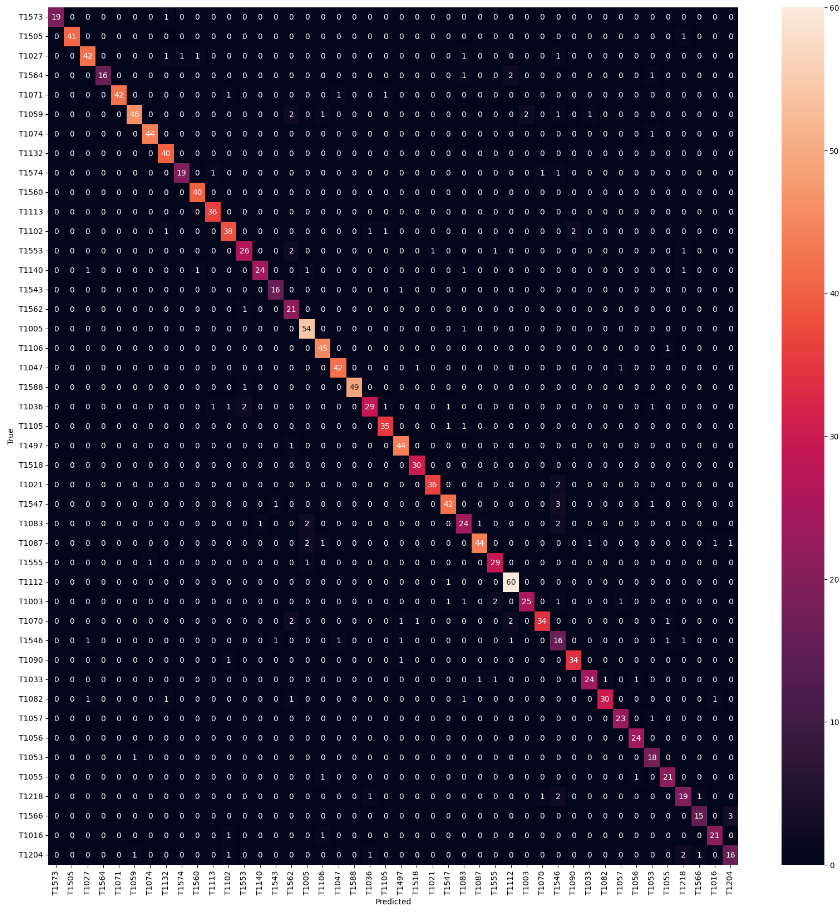
\includegraphics[width=1\linewidth]{scibert_confusion_matrix.png}
    \caption{sciBERT Confusion Matrix}
    \label{fig:cm-scibert}
\end{figure*}
\clearpage
\begin{figure*}[h]
    \centering
    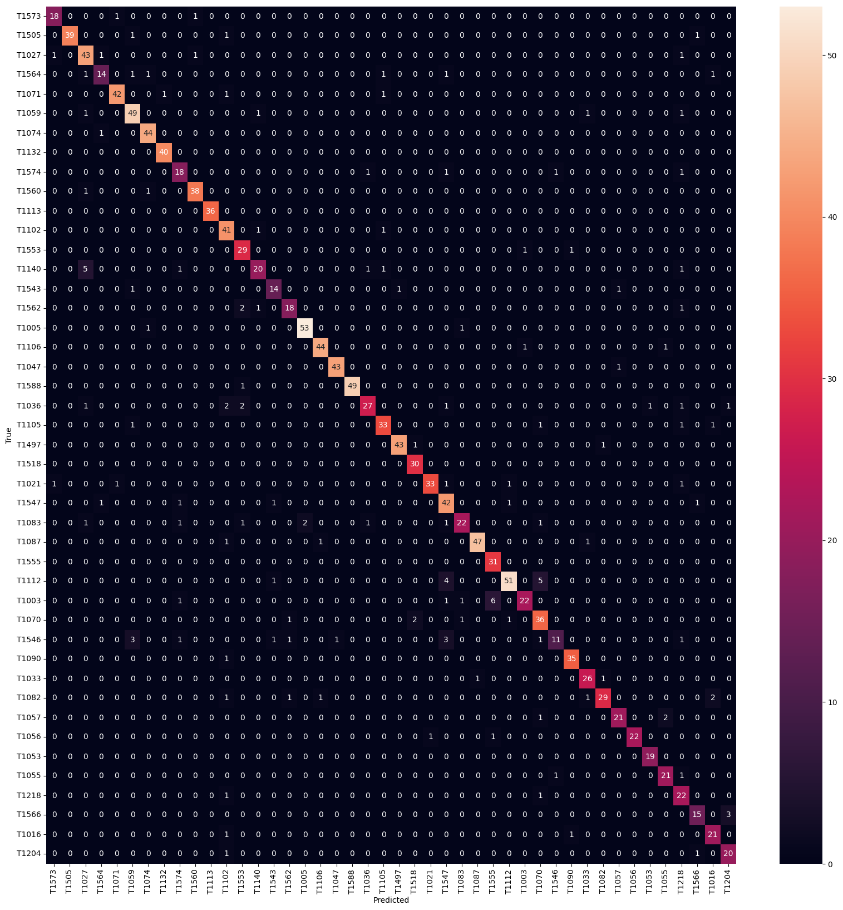
\includegraphics[width=1\linewidth]{secbert_confusion_matrix.png}
    \caption{secBERT Confusion Matrix}
    \label{fig:cm-secbert}
\end{figure*}
\end{document}
